% Candidate research section, 28 October 2026.
% Requires amsmath, amssymb, amsthm; theorem/lemma/proposition definitions supplied by wrapper.
% Independent component review in pfaffian/simplex-equality-audit.md.
\section{The simplex bound through a triangle-free graph}
\label{sec:simplex-sharp}

Haim--Kislev proved the sharp bound $c_{\mathrm{EHZ}}(K)^2/(2\operatorname{vol}_4K)
\leq3/4$ for every four-dimensional simplex in her 2019 MSc thesis
\cite[Theorem~B and Section~4]{HaimKislev2019CubesSimplices}. Her proof
uses pairing coordinates and a substantial sign-case analysis. Later
computations of Chaidez--Hutchings~\cite[Section~1.5]{CH2021} give
equality examples, while Leipold~\cite[Section~12.4]{Leipold2026}
reports numerical simplex values.
We give a different proof: the polar of the four-item linear-ordering
polytope has a triangle-free Pfaffian interaction graph. The graph bound
also yields the complete equality family below. The contribution here is
the proof mechanism and equality description, rather than the numerical
constant or its universal validity.

\begin{theorem}\label{thm:simplex-three-quarters}
Every nondegenerate simplex $K\subset\mathbb R^4$ satisfies
\[
 \frac{c_{\mathrm{EHZ}}(K)^2}{2\operatorname{vol}_4K}\le\frac34.
\]
The constant is sharp. In interleaved symplectic coordinates
$\omega_0=dz_1\wedge dz_2+dz_3\wedge dz_4$, equality holds precisely for
the images under translations, positive dilations and linear
symplectomorphisms of
\[
 K_{\mu,\nu}=\operatorname{conv}\{0,
 (1,0,\nu,-\nu),\ (0,1,-\mu,\mu),\ e_3,\ e_4\},
 \qquad \mu,\nu\ge0,\quad\mu+\nu\le1.
\]
\end{theorem}

\subsection{Barycentric gradients remove the weight optimization}

Let $\lambda_0,\ldots,\lambda_4$ be the barycentric coordinate functions of
$K$, and write $x_i=-d\lambda_i$ for their constant negative gradients,
identified with vectors using the ambient Euclidean coordinates. They obey
$\sum_{i=0}^4x_i=0$, and any four form a basis. Translate $K$ so that the
origin is interior, and set $\beta_i=\lambda_i(0)>0$. Its normalized facet
presentation is
\[
 K=\{z: a_i\cdot z\le1,\ 0\le i\le4\},
 \qquad a_i=x_i/\beta_i.
\]
The unique normalized nonnegative closure vector in Haim--Kislev's formula
is $(\beta_i)$: the kernel of the matrix of the five facet rows is
one-dimensional, and $\sum_i\beta_i=1$, $\sum_i\beta_i a_i=0$.

Define the alternating matrix
\[
 \Omega_{ij}=\omega_0(x_i,x_j),\qquad 1\le i,j\le4,
\]
and the order functional
\begin{equation}\label{eq:simplex-order-functional}
 S(\Omega)=\max_{\sigma\in\mathfrak S_4}
              \sum_{i<j}\Omega_{\sigma(i),\sigma(j)}.
\end{equation}
Closure makes cyclic rotation preserve the ordered pairing sum. Put $x_0$
last; its contribution is
$\omega_0(\sum_{i=1}^4x_i,x_0)=\omega_0(-x_0,x_0)=0$.
The Haim--Kislev formula~\cite[Theorem~1.1]{HK2017} therefore gives
\begin{equation}\label{eq:simplex-capacity-and-volume}
 c_{\mathrm{EHZ}}(K)=\frac1{2S(\Omega)},\qquad
 \operatorname{vol}_4K=\frac1{24|\operatorname{Pf}\Omega|}.
\end{equation}
For the second identity, the affine map
$z\mapsto(\lambda_1(z),\ldots,\lambda_4(z))$ takes $K$ onto the standard
simplex of volume $1/24$. Its absolute Jacobian is the absolute determinant
of the four gradients. The Pfaffian congruence identity gives the same
absolute determinant for $\Omega$. Thus
\begin{equation}\label{eq:simplex-ratio-pfaffian}
 \frac{c_{\mathrm{EHZ}}(K)^2}{2\operatorname{vol}_4K}
 =\frac{3|\operatorname{Pf}\Omega|}{S(\Omega)^2}.
\end{equation}
Conversely, every nondegenerate alternating matrix is a symplectic Gram
matrix of a basis, so this reduction describes the whole affine simplex
class. The gradients determine the labeled simplex up to translation;
equal Gram matrices identify them up to an affine symplectomorphism.

\subsection{The polar of the four-item ordering polytope}

Use coordinates $(12,13,14,23,24,34)$ on the six-dimensional space of
alternating matrices, and let $e_{ij}$ denote its coordinate unit vectors.
In these coordinates,
\[
 q(z):=\operatorname{Pf}z=z_{12}z_{34}-z_{13}z_{24}+z_{14}z_{23}.
\]
For $\sigma\in\mathfrak S_4$, let $p_\sigma$ have coordinate $+1$ on
$ij$ when $i$ precedes $j$ and $-1$ otherwise. Then $S$ is the support
function of $P=\operatorname{conv}\{p_\sigma\}$.

We use the classical facet description of the four-item linear-ordering
polytope: in incidence coordinates $y=(1+p)/2$, it is defined by
\[
 0\le y_{ij}\le1,\qquad
 0\le y_{ij}-y_{ik}+y_{jk}\le1\quad(i<j<k).
\]
After centering and polarity this says
\begin{equation}\label{eq:simplex-order-polar}
 C:=\{z:S(z)\le1\}=\operatorname{conv}\mathcal V,
 \quad
 \mathcal V=\{\pm e_{ij}:i<j\}\cup
 \{\pm(e_{ij}-e_{ik}+e_{jk}):i<j<k\}.
\end{equation}
There are twenty vertices. This small classical polytope identity is the
only ordering-polytope input needed below.
% Classical source: Groetschel--Juenger--Reinelt; Marti--Reinelt Ch.6.
% Independent exact rational active-basis certificate supplied separately.

For completeness, the facet description has a short integrality proof.
Let $R$ be the polyhedron defined by the displayed bounds and triangle
inequalities. At any vertex of $R$, some coordinate bound is active:
otherwise at most one constraint from each of the four triangle pairs can
be active, fewer than the six independent constraints needed at a vertex.
Relabeling the four items, we may suppose $y_{12}=1$. Write
$(a,b,c,d,e)=(y_{13},y_{14},y_{23},y_{24},y_{34})$.
On this face the remaining constraints are the unit box and
\[
 c\le a,\quad d\le b,\quad
 0\le a-b+e\le1,\quad 0\le c-d+e\le1.
\]
The four core row vectors are
\[
 \begin{pmatrix}
 1&0&-1&0&0\\
 0&1&0&-1&0\\
 1&-1&0&0&1\\
 0&0&1&-1&1
 \end{pmatrix}.
\]
Changing their signs by $(+,-,-,+)$ gives a matrix with one $+1$ and one
$-1$ in every column. Every square minor of such a directed-incidence
matrix is $0$ or $\pm1$: expand along a column with at most one nonzero
entry, or, if every column has two, use the zero sum of the rows.
Appending coordinate rows and signed copies preserves this property.
An invertible active constraint matrix consequently has determinant
$\pm1$, and its integer right-hand side forces the vertex coordinates
to be integers. Thus every vertex of $R$ is a zero--one vector. The
triangle inequalities exclude directed triangles; a tournament without
directed triangles is a total order. Hence $R$ is exactly the convex
hull of the twenty-four order vectors, proving
\eqref{eq:simplex-order-polar} without a computational assumption.

\subsection{A triangle-free Pfaffian interaction graph}

Let $f_1,\ldots,f_4$ be the standard basis of $\mathbb R^4$ and
$f_5=f_1+\cdots+f_4$. With the usual Hodge star,
\[
 \mathcal V=\{\pm*(f_i\wedge f_j):1\le i<j\le5\}.
\]
The six pairs not involving $f_5$ give the coordinate vectors; the other
four give the triangle vectors. Every vertex is decomposable and hence
has $q(v)=0$. Define its symmetric interaction with another vertex by
\[
 B(v,w)=q(v+w)-q(v)-q(w).
\]
If $v=\varepsilon*(f_i\wedge f_j)$ and
$w=\eta*(f_k\wedge f_l)$, then
\[
 B(v,w)=\varepsilon\eta\det(f_i,f_j,f_k,f_l).
\]
This is zero when the two index pairs intersect, and is $+1$ or $-1$
otherwise: every four distinct $f_i$ have determinant $\pm1$.

Let $G$ have vertex set $\mathcal V$, with $vw$ an edge exactly when
$B(v,w)=1$. It is triangle-free, since three pairwise disjoint two-element
subsets cannot fit inside a five-element set. It is also cubic: a pair has
three disjoint pairs, and exactly one sign of each gives positive
interaction. These elementary facts already prove the bound.

\begin{lemma}[Triangle-free weighted graph bound]\label{lem:simplex-graph-bound}
If $G$ is triangle-free and $\lambda_v\ge0$, $\sum_v\lambda_v=1$, then
\[
 \sum_{vw\in E(G)}\lambda_v\lambda_w\le\frac14.
\]
\end{lemma}
\begin{proof}
Choose an optimizing weight vector with the fewest positive entries. If
two supported vertices are nonadjacent, redistribute their combined mass
to the one with larger weighted neighbor sum. The objective is linear in
this redistribution, so it does not decrease, contradicting minimal
support. The support is therefore a clique, of size at most two. Its
edge contribution is at most $t(1-t)\le1/4$.
\end{proof}
This is the triangle-free case of the Motzkin--Straus
theorem~\cite[Theorem~1]{MotzkinStraus1965}; its short
proof is included to make the numerical constant transparent.

\begin{proof}[Proof of Theorem~\ref{thm:simplex-three-quarters}]
For $z\in C$, write $z=\sum_v\lambda_vv$ as a convex combination of
vertices in~\eqref{eq:simplex-order-polar}. Since $q(v)=0$,
\[
 q(z)=\sum_{v<w}\lambda_v\lambda_wB(v,w)
 \le\sum_{vw\in E(G)}\lambda_v\lambda_w\le\frac14.
\]
An odd permutation of the four coordinate indices preserves $S$ and
reverses the Pfaffian sign. Applying the same argument after such a
permutation proves $|q(z)|\le1/4$ on $C$. Homogeneity gives
$4|q(\Omega)|\le S(\Omega)^2$; now use
\eqref{eq:simplex-ratio-pfaffian}. The standard simplex has
$c_{\mathrm{EHZ}}=1/4$ and volume $1/24$, giving equality.
\end{proof}

\subsection{All equality forms}

Two distinct vertices of $G$ have at most one common neighbor. To see this,
forget signs and label a vertex by its two-element subset of
$\{1,\ldots,5\}$. Two distinct subsets have at most one common disjoint
pair. If the signed vertices have the same underlying subset, they have
opposite signs and no common positive neighbor. Thus $G$ has no
four-cycle. Its unsigned quotient is the Petersen graph. Only the
established absence of triangles and four-cycles is used below.

\begin{figure}[tb]
 \centering
 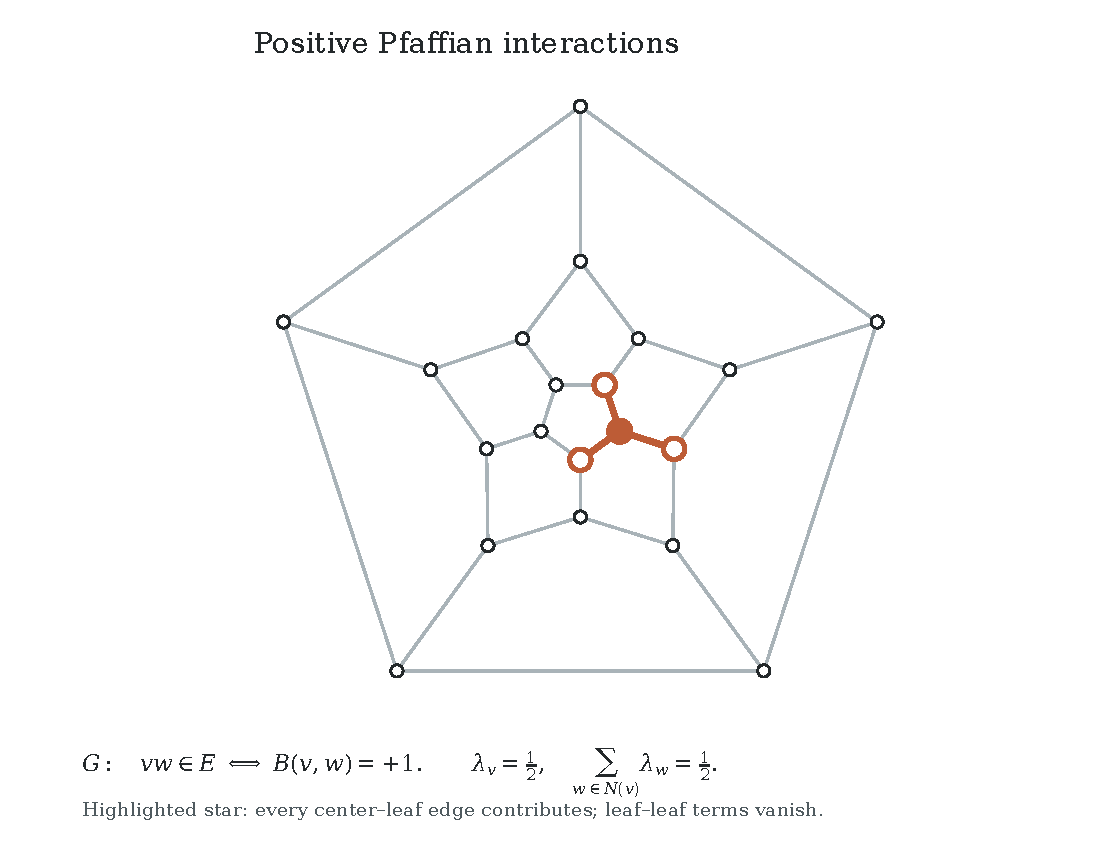
\includegraphics[width=.83\linewidth]{figures/pfaffian-graph.pdf}
 \caption{The positive-interaction graph on signed rank-two vertices.
 The highlighted star shows an equality support: half the mass is at its
 center and half is distributed among its three neighbors.}
 \label{fig:pfaffian-graph}
\end{figure}

\begin{proposition}\label{prop:simplex-equality-locus}
The set $\{z:S(z)=1,\ q(z)=1/4\}$ is exactly
\[
 \bigcup_{v\in\mathcal V}
 \left(\frac12v+\frac12\operatorname{conv}N_G(v)\right).
\]
Each $N_G(v)$ consists of three vertices, so this is a union of twenty
closed triangles. Negative-Pfaffian equality is obtained by any odd
coordinate permutation, and positive scaling gives all nonzero equality
forms.
\end{proposition}
\begin{proof}
Suppose $q(z)=1/4$ and choose a convex decomposition
$z=\sum_v\lambda_vv$. Both inequalities in the preceding proof are
equalities. The weights maximize the graph quadratic at $1/4$.
On their positive support, first-order variations show that all weighted
neighbor sums are equal. Their weighted average is twice the objective,
so each is $1/2$.

Choose a supported edge $uv$. The supported neighbor sets of $u$ and $v$
are disjoint, by triangle-freeness, and each has mass $1/2$. They therefore
partition the support. Each side is independent. Every vertex must be
adjacent to the whole opposite side, since its weighted degree is $1/2$
and every supported weight is positive. The support is complete
bipartite. The absence of four-cycles forces one side to be a singleton:
the support is a star, its center has mass $1/2$, and its leaves have total
mass $1/2$.

Conversely, any two neighbors of a vertex have underlying pairs in the
same remaining three-element set. They intersect, so their interaction
$B$ is zero. Every such balanced star therefore has Pfaffian $1/4$.
It lies in $C$; the proved inequality forces $S=1$.
\end{proof}

For example, the positive neighbors of $e_{12}$ are
\[
 e_{34},\qquad e_{13}-e_{14}+e_{34},\qquad
 e_{23}-e_{24}+e_{34}.
\]
Doubling this equality triangle gives the explicit family
\[
 \Omega=e_{12}+e_{34}
       +\mu(e_{13}-e_{14})+\nu(e_{23}-e_{24}),
 \qquad \mu,\nu\ge0,\quad\mu+\nu\le1,
\]
with $q(\Omega)=1$ and $S(\Omega)=2$. The union in the proposition is the
complete equality classification in pairing coordinates.

To pass from twenty triangles to the family in the theorem, relabel the
five barycentric gradients. If $B_\pi$ expresses the new four-vector basis
in the old one, the induced action is
$\Omega\mapsto B_\pi^T\Omega B_\pi$. It preserves $S$, and
$\det B_\pi=\operatorname{sgn}\pi$. An odd relabeling first makes the
Pfaffian positive. The even relabelings act transitively on $\mathcal V$:
even permutations fixing the omitted label give all twelve signed
coordinate vectors from $e_{12}$; exchanging the omitted label with a
third index, and exchanging the first two indices to preserve parity,
gives the eight signed triangle vectors. They therefore take any
equality triangle to the displayed one. Scaling then sets $q=1$.

For an explicit realization, let $X$ have columns
\[
 e_1,\ e_2,\ -\nu e_1+\mu e_2+e_3,\
 \nu e_1-\mu e_2+e_4.
\]
Then $X^T JX$ is the displayed $\Omega$, and $X^{-T}$ has columns
$(1,0,\nu,-\nu)$, $(0,1,-\mu,\mu)$, $e_3$, $e_4$.
The negative barycentric gradients of $K_{\mu,\nu}$ are the negatives
of the columns of $X$, together with their opposite sum. Hence this
simplex has the required pairing matrix. It has volume $1/24$ and
capacity $1/4$. Equal pairing matrices give affine symplectomorphisms,
so every equality simplex has the stated form up to the claimed
transformations.

The parameter boundary has a geometric meaning. The ten pairings of the
five weighted facet normals have absolute values
$1,1,1,1,\mu,\mu,\nu,\nu,1-\mu-\nu,1-\mu-\nu$.
An intersection of two facets is Lagrangian exactly when their normal
pairing vanishes. Thus interior parameters give equality simplices with
no Lagrangian two-faces, open edges give two, and the three corners give
four. Thus the equality family contains simplices with no Lagrangian
two-faces, as observed experimentally by Chaidez and Hutchings.
